\section{图形化Nsight Compute使用}

在前文中，讨论了 Nsight Compute 工具的命令行分析。其中提到有两种方法来分析任何 CUDA 应用程序。第一种是使用命令行分析，前文已经讨论过了，其中讨论的一些分析内容是本节所需要的。第二种方法是使用 Nsight Compute 工具的图形用户界面，这就是本章的主要内容。将探索 Nsight Compute 的图形界面，即 GUI。照例，这是文档链接。需要说明的是，有两份文档，不是一份。一份是关于 Nsight Compute 工具图形界面的；另一份是关于命令行分析的。

\subsection{安装与项目创建}

当打开一个新项目时，需要编辑一些配置，以便能够对 CUDA 应用程序进行性能分析。完成初始步骤后，需要查看输出。但在那之前，需要确保系统上已经安装了这个工具，无论使用的是 Linux 还是 Windows 操作系统。如果系统上没有安装 Nsight Compute 工具，安装起来非常简单。

当安装 CUDA 时，CUDA 工具包包含了所有内部工具，例如 Nsight Compute 或 Nsight Systems 等。搜索 "Nsight Compute tool for Windows"，打开第一个链接，点击这里。它可能会要求在 NVIDIA 网站注册，可以使用任何电子邮箱进行注册。注册后，会看到这个网页，可以从这个链接下载 Nsight Compute。安装过程非常简单。然后搜索 Nsight Compute，打开工具。

\begin{figure}
    \centering
    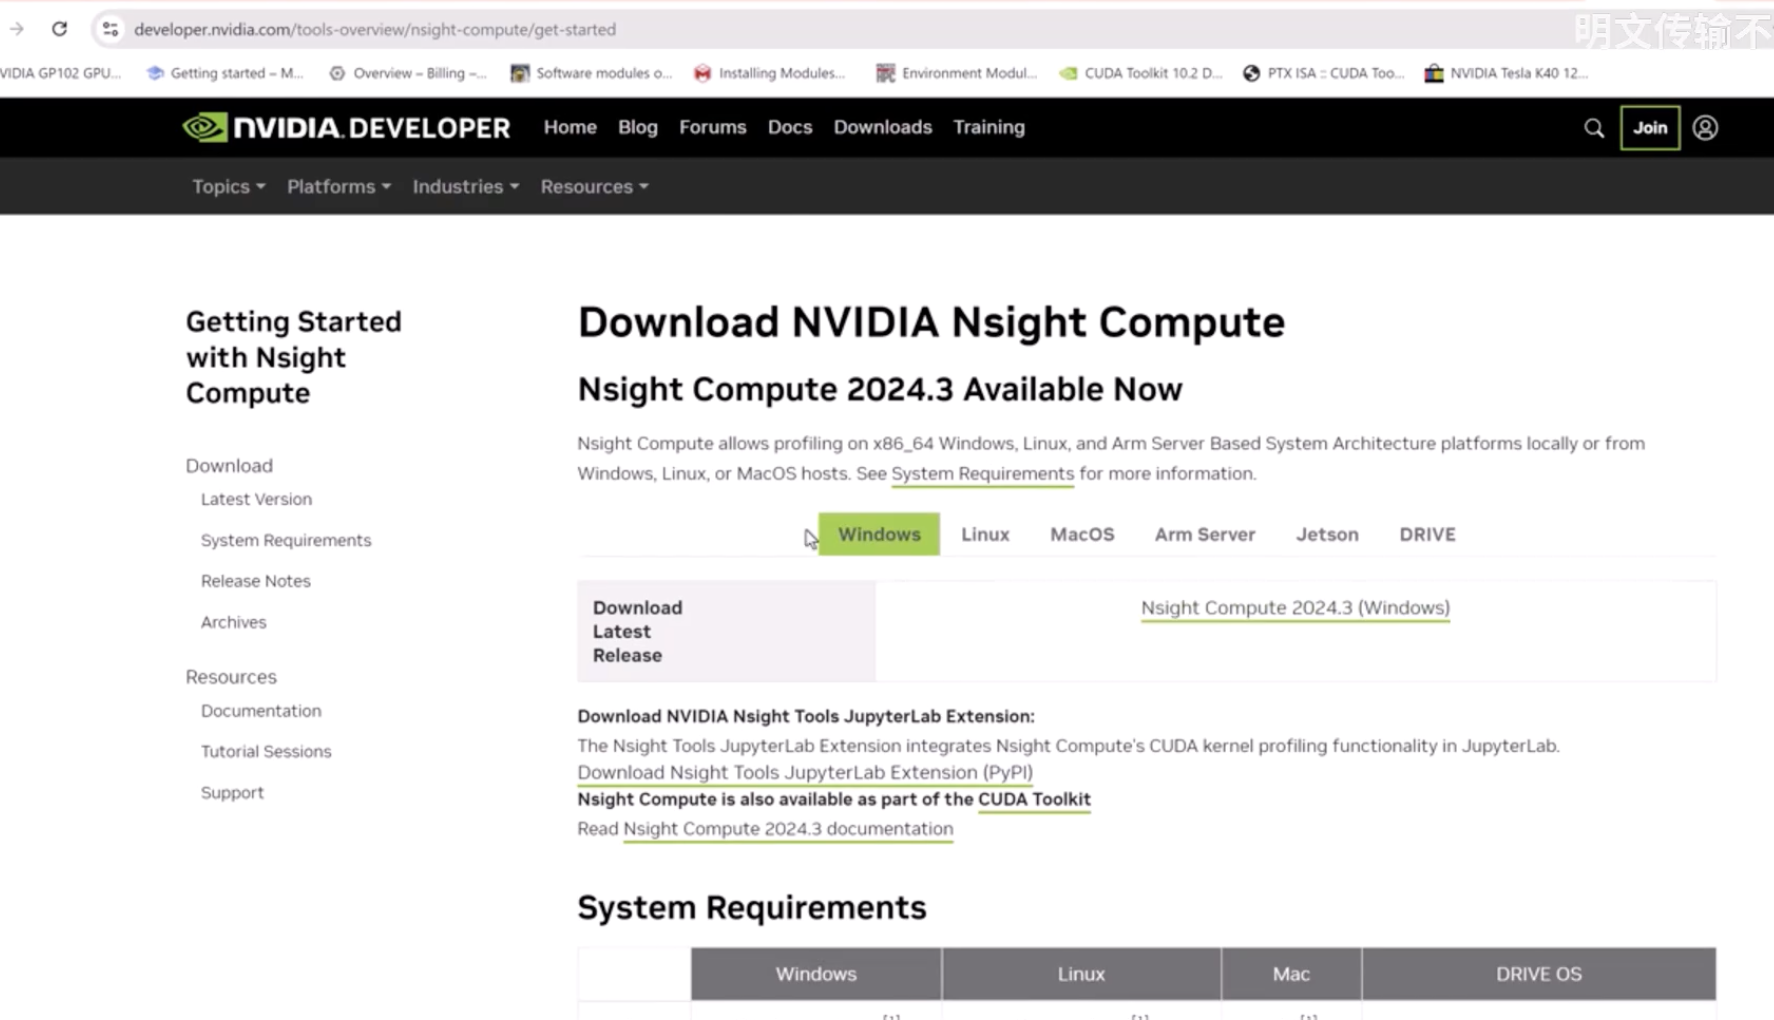
\includegraphics[width=0.75\linewidth]{resources/cuda-105.png}
    \caption{}
    \label{fig:placeholder}
\end{figure}

这里有两个版本，一个是 24.11，第二个是 24.3.2。将打开这个版本。

它是这样启动的，有一些选项，可以打开一个文件、创建一个新项目，或者加载一个已有的项目。这些是 Nsight Compute 图形界面最近的一些增强功能。

需要做的只是从文件菜单打开一个新项目。但在那之前，需要知道 CUDA 应用程序的确切位置。这是 CUDA 课程的文件夹，这是第四节的文件夹。如所示，这里有一些 CUDA 应用程序，还有可执行文件。但在那之前先编译这个 CUDA 应用程序，输入 \texttt{ls}。

有一些 \texttt{.cu} 文件，还有之前章节生成的可执行文件。但今天需要做的是生成带 \texttt{.exe} 扩展名的可执行文件。使用 NVCC 编译器，写例如 \texttt{-o}，这是为了保存编译过程的输出。随便起个名字，例如就叫 \texttt{aa.exe}。

这是可执行文件，这是 CUDA 文件。这个命令会生成这个可执行文件。如所示，这里还没有这个可执行文件。按回车键，然后输入 \texttt{ls}。如所示，这里有了可执行文件。然后回到这里，点击新项目，给它起个名字，点击确定，这里就是配置项。只解释主要的几个。例如这个选项是必须的，这是应用程序可执行文件，已经用这个命令生成了，从这里选择。

复制路径，选择 \texttt{aa.exe} 文件打开。如所示，感叹号被移除了。然后可能需要选择工作目录，例如选择第四节文件夹。

从这里开始有一些配置，比如说是否想启用 CPU 调用栈？是否想启用对 CPU 和 GPU 通信的性能分析过程？如何处理缓存？需要在时钟控制中刷新它们全部。刷新的意思是清除先前存在于缓存中的所有内容。

需要使用基础频率还是无基础？这将指 GPU 的基础时钟频率。对于图分析需要使用节点 1。如果想了解更多，可以从这里查阅文档。

如果现在点击立即启动，它是不会工作的。因为需要开始执行这个应用程序，才能对其进行分析。将添加附加（Attach），可以看到进程名，这里没有任何进程，可以通过这个命令来做到。需要来到这里并开始执行，以便从 CPU 到 GPU 创建一个新进程。

这个命令叫做 \texttt{ncu}。将使用的模式是 \texttt{--launch-mode attach}，然后是 \texttt{./aa.exe}。

那个模式意味着需要让 GPU 开始执行，但它不应该结束。因为需要分析，需要一个正在运行的进程。当按回车键时，例如 \texttt{./aa}，如所示它执行了。但当使用这个命令时，它只是启动了一个进程，消耗了大约 8.2 毫秒。可以通过点击这里的附加来完成。现在可以将这个进程附加到 Nsight Compute UI。

如所示，\texttt{aa.exe} 可以显示在这里，这是进程 ID。先按 Ctrl+C 取消，然后来到这里。

点击附加，再点击这个。需要将参数改为对应的值，因为这是今天的应用程序。点击这个，然后点击附加。现在可以附加了，或者可以来到这里点击启动，如所示一切运行正常。现在需要看看左侧有什么。但它现在是空的，因为还没有开始性能分析。

\begin{figure}
    \centering
    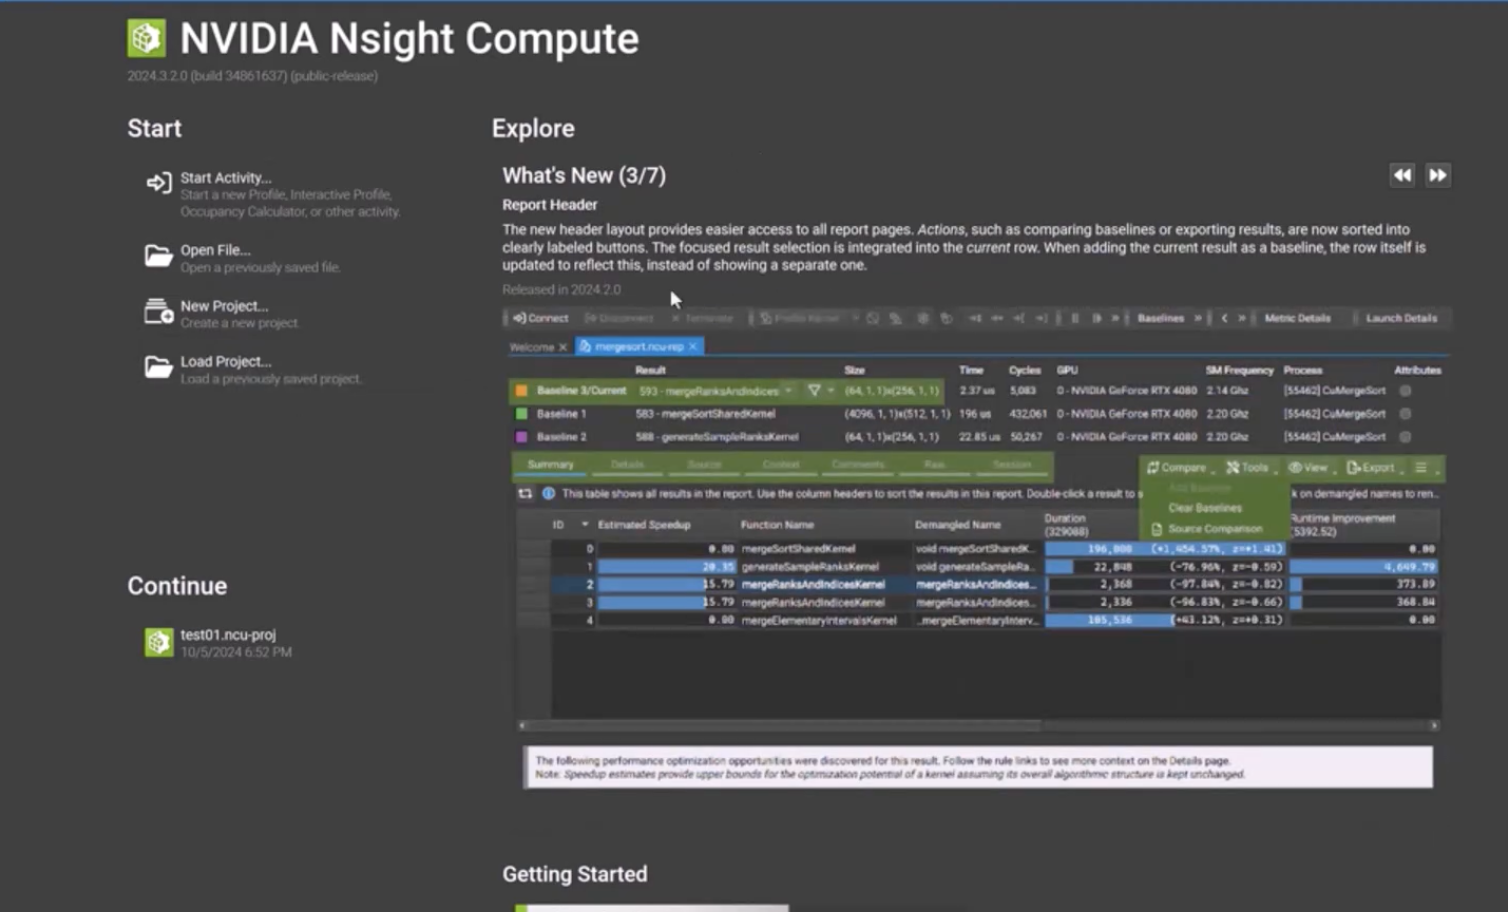
\includegraphics[width=0.75\linewidth]{resources/cuda-106.png}
    \caption{}
    \label{fig:placeholder}
\end{figure}


\subsection{附加进程与指标选择}

在下面的标签页中，可以看到一个叫"指标选择"、"API 统计"的标签页。只是附加到了进程，但还没有开始分析本身。如何开始分析呢？在指标选择中，可以选择任何想要分析的项目，即需要分析哪些指标，需要做哪些性能分析。

从这里开始，选择所有与 Speed of Light 相关的内容，例如 Speed of Light 吞吐量、Speed of Light 屋顶线图（Roofline）、Speed of Light 分层屋顶线图等。如果点击这里，可以看到其他一些选项。同时不选择 PM 采样，但选择计算工作负载（Compute Workload）。如果只想要这些选项中的一个，可以选择它。然后可以在这里选择所有已选的选项，因为它们都非常重要，后面将解释每一个。然后也可以选择指令统计、启动统计、占用率（Occupancy）、GPU 和内存工作负载分布等。

如果还记得之前的讨论，会知道在这里选择的项目在命令行分析中是以部分（Section）的形式呈现的。例如还记得前文中的表格吗？这些就是 Nsight Compute 中包含的部分。

例如看计算工作负载分析，如果来到这里，可以看到计算工作负载分析，然后看一下，例如 Sub-warp 统计。然后再回到这里，会看到 Sub-warp 统计。一旦为分析过程选择了所需的部分和指标，就可以来到这里。同样适用于调度器统计、内存工作负载分析等。然后可以开始点击这里"运行至下一个核函数"。

VectorAdd，这是下一个核函数。选择核函数，然后点击分析核函数，这就是分析过程的开始。一旦点击分析核函数，它将开始执行应用程序，并在执行过程中收集性能指标。

\subsection{分析结果概览}

如所示，分析过程已经完成，可以查看结果了。这里没有结果，因为有很多标签页需要选择。例如有一个摘要（Summary），从这个摘要中可以看到一些信息：已实现的占用率。它解释了理论占用率和已实现占用率。例如理论占用率是 100\%，前文已经讨论过这个了。在命令行分析中的占用率，理论占用率是 100\%，已实现的占用率大约是 80\% 或 81\%。

使用的是相同的指标，但显示指标的方式不同。这里通过一些信息图表来显示，而那里是通过表格来显示的。如果来到这里，可以看到同样的理论 100\%，已实现 81\%。也可以看到这些内容并阅读，但将从另一个标签页阅读。

那个标签页有更多细节，例如详情（Details）标签页，如所示，这里会显示包含的所有部分。例如 GPU Speed of Light 吞吐量，这是第一个；然后有计算工作负载分析；然后是内存工作负载分析。这里有一些技巧可能会给出更多信息，因为可以看到一些表格。

在指标选择中包含的所有内容，都会在详情标签页的这个部分看到其输出。组织得很好。例如可以看到吞吐量，有 16\% 的吞吐量。同样可以再次回到命令行分析，看到这个值也显示在那里。这里只是在两种方法之间建立联系，以便选择最适合的方法。

先看这里，内存吞吐量是 95\%，L1 和 L2 缓存的吞吐量分别是 21\% 和 40\%。在这里可以看到经过的周期数，这个核函数执行的持续时间等。此外如果选择这些选项或指标中的任何一个，可以在这里看到细节。例如，如果在这里选择持续时间，它会显示单位，单位是纳秒，显示值。这里的值是 970，也就是 978，但这里是纳秒，那里是微秒。如果想在命令行分析中做同样的事情，可以使用这个指标。

如所示，\texttt{gpu\_\_time\_duration}。还记得那个分析吗？所有想从图形界面获取、以便于命令行分析一起使用的内容，都可以从这里获取。然后在这个右侧部分的末尾，可以看到 Average、Sum、Minimum。这些在前文中也讨论过。

现在可能会问，为什么最小值、最大值、总和所有这些都有相同的值？因为现在讨论的是持续时间，而对于整个 GPU 的时间，它们应该是相同的。但对于其他情况则不同，例如周期数，每个 SM 使用的字节数就不同。但讨论的是总时间，总时间它们应该相同。

这是第一部分，GPU Speed of Light 吞吐量。然后这里有计算工作负载分析。如所示，有每个周期的指令数（IPC），每个活动周期的指令数，需要搜索它们之间的区别，这是经过的（Elapsed），这是活动的（Active）。这些将在后续章节中讨论。

但这不是本节的重点，因为本节的主要重点是熟悉 Nsight Compute 工具，而不是优化应用程序，也不是理解每个术语。重点是理解 Nsight Compute 工具。在其他章节中将使用 Nsight Compute 工具进行优化。

\begin{figure}
    \centering
    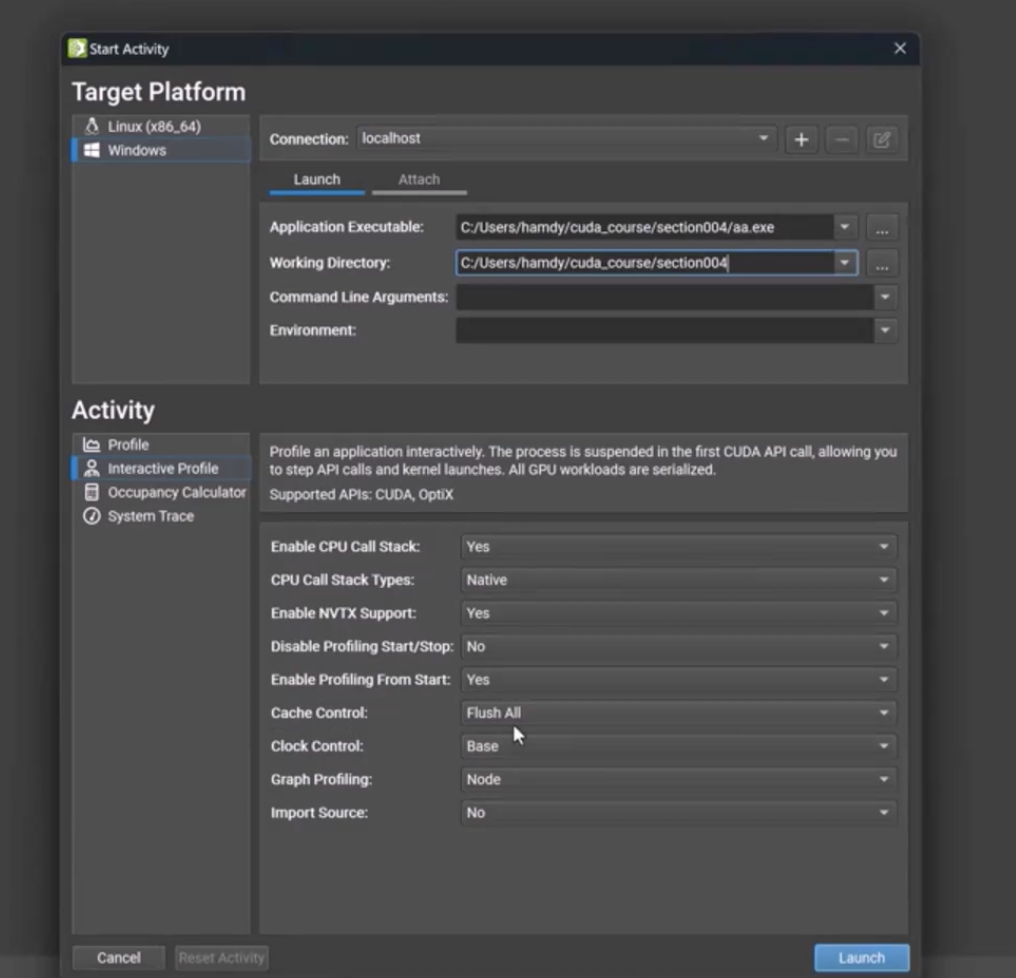
\includegraphics[width=0.75\linewidth]{resources/cuda-107.png}
    \caption{}
    \label{fig:placeholder}
\end{figure}


\subsection{内存瓶颈分析}

接着还有内存工作负载，这里有 SM 繁忙时间的百分比。这里有 L1 的命中率，有 0\% 的命中率。在命令行分析章节中测量过这个，33\% 的命中率，这也非常糟糕。对于 L2 命中率有 33\%，这意味着在内存操作上消耗了太多时间或太多周期。因为必须访问 L1，却找不到需要的数据。然后访问 L2 能找到一些，但其他的数据不在那里。需要从全局内存进行大量读取甚至写入操作，这需要很长时间，需要很多周期，数百个周期。这里只是逐步说明这些数字的含义。

然后有内存繁忙百分比、最大带宽，实现了大约 95\% 的内存带宽。有 95\%，现在可能会想这很好，是个好兆头。但这并不好。因为如果实现了全局内存最大带宽的 95\%，这意味着访问全局内存太频繁了，需要减少这种情况。

理解这些指标的含义非常重要。再看看 L2 缓存中包含了一个叫做压缩的功能，这与 Ampere 架构也有关系。因为这些功能中的一些是从 Ampere 架构开始引入的，而不是之前的架构，比如 Volta、Turing、Pascal 等。然后还有调度器统计，前文已经讨论过调度器统计了。

在讨论 Sub-warp 统计之前，先停在这里。可能会问，这些表格看起来和这里的表格非常相似，简直一模一样。在这里做什么？命令行分析和图形用户界面之间有什么区别？它们显示的是相同的表格吗？但事实并非完全如此。稍后将跳转一下，展示图形用户界面中包含的最佳功能。

这里有 Sub-warp 统计，如所示，有一个非常重要的指标：每个已发布指令的 Sub-warp 周期数。需要阅读所有这些信息。可以说大约需要 119 或 120 个周期来处理每个已发布的指令，这非常重要。需要阅读所有内容，因为这些说明中的一些可以看作是对你的建议或者是一些要点，能帮助优化应用程序以实现高性能。

例如读一下这里的说明："平均而言，这个核函数的每个 Sub-warp 大约花费 111 个周期处于停滞（Stall）状态。"这非常糟糕。停滞意味着这个 Sub-warp 在约 111 个周期内什么都没做。想象一下，有 111 个周期，每个 Sub-warp 就只是停在那里不退出，也不执行任何指令。如果继续看会找到导致这个问题的原因。需要改进这一点，以确保在每个周期内尽可能让每个 Sub-warp 执行一些操作，执行一条指令。

这背后的原因是什么？说过有 111 个周期的停滞。"等待长计分板依赖（Long Scoreboard Dependency）"，可以阅读来了解，这里的依赖意味着某个指令正在等待前一个结果或从内存的读取操作。它说明依赖是由于从 L1/纹理缓存读取数据，或者可能是来自其他内存层级。例如本地内存、全局内存、表面内存或纹理操作单元。可以从这里知道遇到了内存瓶颈问题。

\begin{figure}
    \centering
    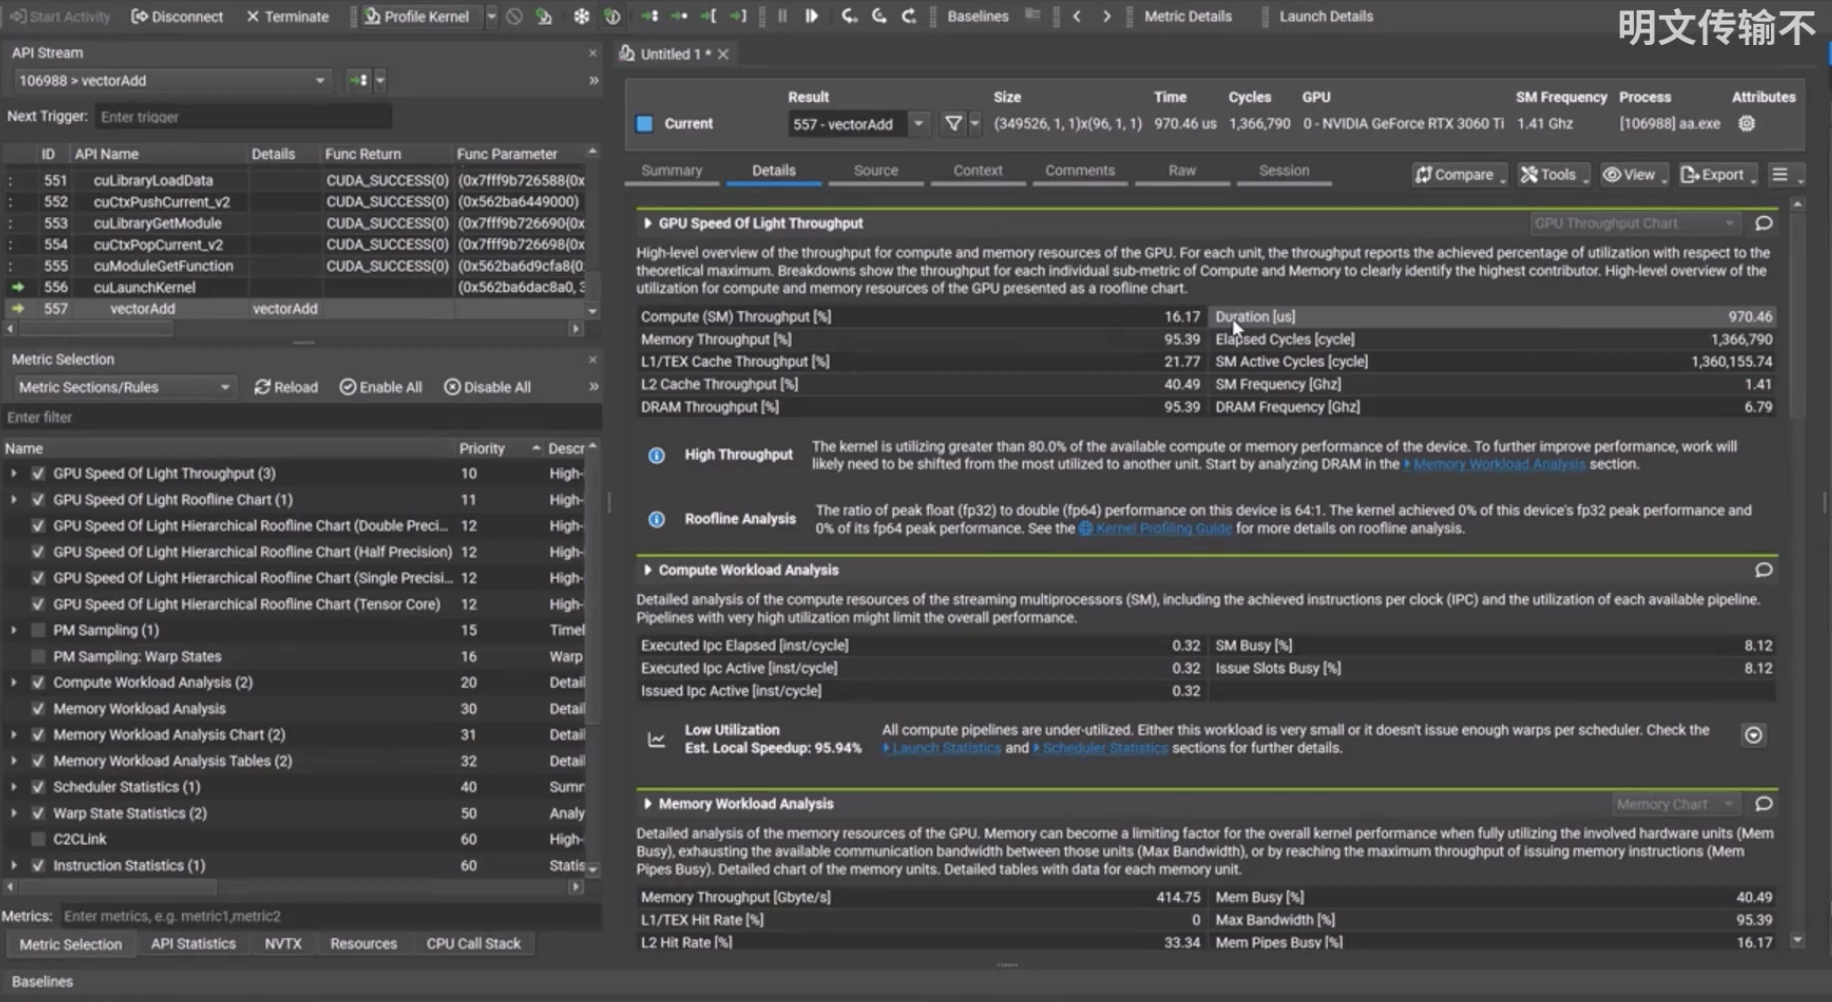
\includegraphics[width=0.75\linewidth]{resources/cuda-108.png}
    \caption{}
    \label{fig:placeholder}
\end{figure}

\subsection{源代码与汇编分析}

回到这里，还记得最大带宽吗？当说如果正在实现一个高带宽时，高内存带宽在某些情况下可能是好的，但在其他情况下就非常糟糕。这就是这些指标与在 Sub-warp 统计中看到的停滞是如何关联的。特别是当 L1 和 L2 命中率很低时。然后可以看到每个 Sub-warp 有 32 个线程，每个 Sub-warp 有 30 个未被屏蔽（Unmasked）的线程。

继续看查找产生数据的指令。但在那之前来到这里，点击视图标签页，然后点击这里的展开所有部分。它说需要找到导致停滞的指令，下面展示这一点。如所示，这就是图形用户界面和命令行分析之间的主要区别。这是添加到 Nsight Compute 图形界面中的最佳功能。看到这个部分了吗？如所示，拥有相同的部分。除了图表之外，这里没有添加任何新内容。

看到计算工作负载了吗？看到内存工作负载了吗？可以很容易地阅读它，但添加了一些图表，以便用一种好的方式将数据或分析输出可视化。

例如，这里有两个重要的吞吐量或利用率计算：SM 吞吐量和内存吞吐量。说过内存吞吐量是 95\%。但计算吞吐量是多少呢？16\%，这意味着这个应用程序是内存瓶颈型（Memory Bound）的，为什么？因为它只使用了 16\% 的算术逻辑单元（ALU）。只利用了 16\%，但从内存方面利用了 95\%。

这意味着应用程序大部分时间在进行内存操作，而不是算术运算。不需要这样，需要在提高 L1 和 L2 命中率的同时，稍微降低这个数值。因为如果提高了 L1 和 L2 的命中率，那将减少内存带宽的使用。同时增加算术运算，以充分利用可用的硬件核心。这就是如何解释内存瓶颈或者说应用程序的瓶颈——它是计算瓶颈型（Compute Bound）还是内存瓶颈型。

这是第一个图表，非常重要。也可以阅读这两条说明，因为可能会给出一些启发。也可以点击这些链接，一些是在线的。如果点击这里，这将带你到内存工作负载分析部分。

看看计算工作负载分析。如所示，这只是对不同类型算术操作及其利用率的可视化呈现。例如这里有 FMA 单元或 FMA 指令。FMA 指的是融合乘加运算（Fused Multiply-Add），而 ALU 则包含除双精度外的所有其他算术操作。这将包括例如单精度、半精度、整数精度等。这里使用了大约 3.55\% 的可用资源用于融合乘加运算。

而这里使用了大约 4\% 左右，但这指的是活动周期中的百分比，意思是如果整个 GPU 有 100 万个活动周期，大约使用了其中的 4\% 来执行 ALU 运算。另外 4\% 或 3.55\% 用来执行乘加运算。

后面将给出一个关于这个的实际例子。这里有其他单元，例如加载/存储单元（LSU）。不确定 IDU 指的是什么，但双精度在这里。无论如何，这是相对于执行的峰值指令数而言的。意思是从白皮书中知道，在这款 GPU 这个架构上，不同类型的算术操作有一个可执行数量的峰值。假设例如加载/存储单元的峰值是 1000 TOPS。这里只使用了峰值数的 16\%。可以看到这里执行了太多的加载和存储单元指令。

加载和存储单元执行什么操作？内存操作、全局内存、L1/L2 内存操作或者共享内存操作。如果把它与 ALU 和 FMA 相比，这并不好。可以看到，这个单元的待执行指令数量很大。而这是因为如果内存操作相比 ALU 来说很大，这将导致内存瓶颈。

看看内存工作负载分析，这非常重要。因为它会给出一个概念，并提供更多关于有多少请求、在不同内存层级之间移动了多少数据等细节。这里没有使用任何单精度或双精度，这就是为什么它们都是零。

这里有主要的内存单元，例如有共享内存加载、全局内存存储、共享内存。这是稍后会讨论的单元，先别关注它。另一个单元叫做表面内存、纹理内存、本地内存和全局内存。这是第一级，这里有它们的第一级。还记得命令行分析吗？\texttt{l1tex\_\_...}，这是 L1 缓存。还记得这些指标以及它们是怎么写的吗？如所示，它们显示命中率是 0\%。

从这个图形界面可以读取许多性能指标，而无需费力去阅读指标名称、硬件单元名。需要提醒一下，看到这个了吗？有十万个指标，还记得吗？

这里一切都组织得很好。这比试图搜索需要知道的指标在哪里、描述是什么等要好得多。如所示，L1 缓存的命中率是 0\%。对于共享内存没有请求。因为在这个应用程序中，如果没有使用共享内存，只是在不使用任何共享内存的情况下将两个向量相加。这就是为什么这里的请求数量是 0。

然后是第二级 L2 缓存，这里是零或者说是 33\%。如所示，在它们之间有传输的数据量，可以计算所有这些。然后从 L1 到 L2，这意味着写入结果，因为正在读取向量 A 例如从 L2 到 L1，移动了大约 268 兆字节和向量 B，然后计算单元将完成执行，写入的数据量大约是此值的一半。因为读取两个向量，但只写入一个向量即 C 向量。然后 L2 缓存中的命中率是 33\%。

接下来给你一个任务，需要搜索如何提高 L2 缓存的命中率。只是思考一下，看看是否能做些什么。然后这是设备内存，也就是最后一级。有全局内存、L2 缓存、L1 缓存以及计算单元本身之间的请求数量。这来自 ALU，来自 SM。而内存单元会将这些操作发送到 L1 级。大约有 315 万条指令从 SM 发出，到达加载和存储单元或全局内存操作单元。

然后 L1 级如果没有命中，会将这些请求发送到 L2。L2 如果命中，它会将结果或数据发送回这里。如果没有命中，它将向设备内存请求这个数据。这里展示的就是这个情况。这就是内存图表图形界面的样子。大约有 100 万次请求从 SM 发往 L1，大约有 210 万次对这些请求的回复。

如所示，不太确定具体如何解读。这里说例如如果看到这个颜色，这意味着正在达到峰值。例如看这里，如果记得设备内存的吞吐量是 95\%，可以看这里，用了这个颜色。因为有 95\%，但对于 L2 有 33\%。

这就是为什么它在这个区域是这个颜色。对于 L1 有 0\%，它是深色的。如所示，这是一个非常重要的图表。然后这里有调度器统计。再次建议阅读这里的所有内容，GPU 每个调度器最大 Warp 数，如果记得应该是 16。

在这个应用程序中实现了 12 个，有一个不错的值。如果有 16 个，而实现了 12 个，这很好。这是每个调度器的理论值，数值也是 12。每个调度器的活动 Warp 数大约是 9.69，这是理论的，这是实际达到的。然后每个调度器的合格（Eligible）Warp 数和每个调度器已发出的 Warp 数。总之现在不关注所有这些，这里相同的数据用图表可视化了。

如所示长时间计分板停滞（Long Scoreboard Stall），大约是 111 个周期停止等待。可以查看这个 Warp 采样。搜索一下长时间计分板停滞。但不管怎样，这里有短时间计分板停滞（Short Scoreboard Stall）。

这是指如果命中了某个内存层级，但这是指如果计算所有层级的平均值。然后有指令统计。这与不同的指令有关，停滞、耗尽（Throttle）、选定存储屏障。需要查找更多关于这些类型停滞的信息。例如整数乘加指令，意思是所有这些指令都在这个应用程序中执行了。并且获取每一条汇编指令，试图告诉你每条指令在应用程序中执行了多少次。

例如看乘加指令，可以看到它执行了超过 400 万次。\texttt{S2R} 这是用来读取时钟之类的，大约是二百多万次。有一个从内存加载值的加载指令，如所示，它也执行了超过 200 万次。移动指令超过 200 万次，退出指令等。还有将两个值相加的 \texttt{IADD} 指令，执行了一百多万次。

如果想查看这个应用程序中的所有指令，可以转到源代码（Source），这是这个应用程序核函数的汇编语言。这是汇编语言，这是 CUDA 的代码。这是这个核函数的汇编语言。还记得这里的内容吗？

需要加载 A 值，然后加载 B 值，将它们相加并将结果存储在 C 中。这里读取线程 ID、块 ID 并进行一些计算，比如加法和乘法，并将值存储在 i 中。这里使用 i 值从内存加载 B、从内存加载 A、将两个值相加，并将结果存储在 C 中。这就是将在汇编语言输出中看到的内容。

例如看看这个，还记得这个指令吗？这只是读取一个寄存器，一个预定义的寄存器，如所示这个值线程 ID，这个值 CTID，前文中说过 CTA 指的是块 ID。一旦读取了线程 ID 和块 ID，如果还记得这里，需要进行加法和乘法。这就是为什么这里有 \texttt{IMAD}。\texttt{IMAD} 指令将在这里执行，这里还有另一个 \texttt{IMAD}。一旦通过 \texttt{IMAD} 计算完所有这些值，需要将它们存储在这个值即 R6 值中，这就是 i 变量。然后有 \texttt{EXIT}，因为 if 语句的条件没有满足，那么需要退出。

如果 i 不小于 N 需要退出核函数，然后需要执行 if 语句。这就是在汇编语言中做 if 语句的方式。但如果不是，如果 i 小于 N 需要执行这个，这就是为什么这里有 \texttt{EXIT} 指令。如果达到了语句的条件，意思是需要执行这里的这个命令，那么将执行 if 语句内部的内容。

如所示，不会看所有的指令。但这里是前几条指令，前四条指令只是获取 i 值。需要在这里做的是有一个加载 A 的指令，一个加载 B 的指令。这是从内存加载，这也是从内存加载，然后需要乘加。因为一旦加载了 B 和 A 需要将两个值相加。这就是为什么需要 \texttt{IMAD} 或 \texttt{ADD} 指令。

\begin{figure}
    \centering
    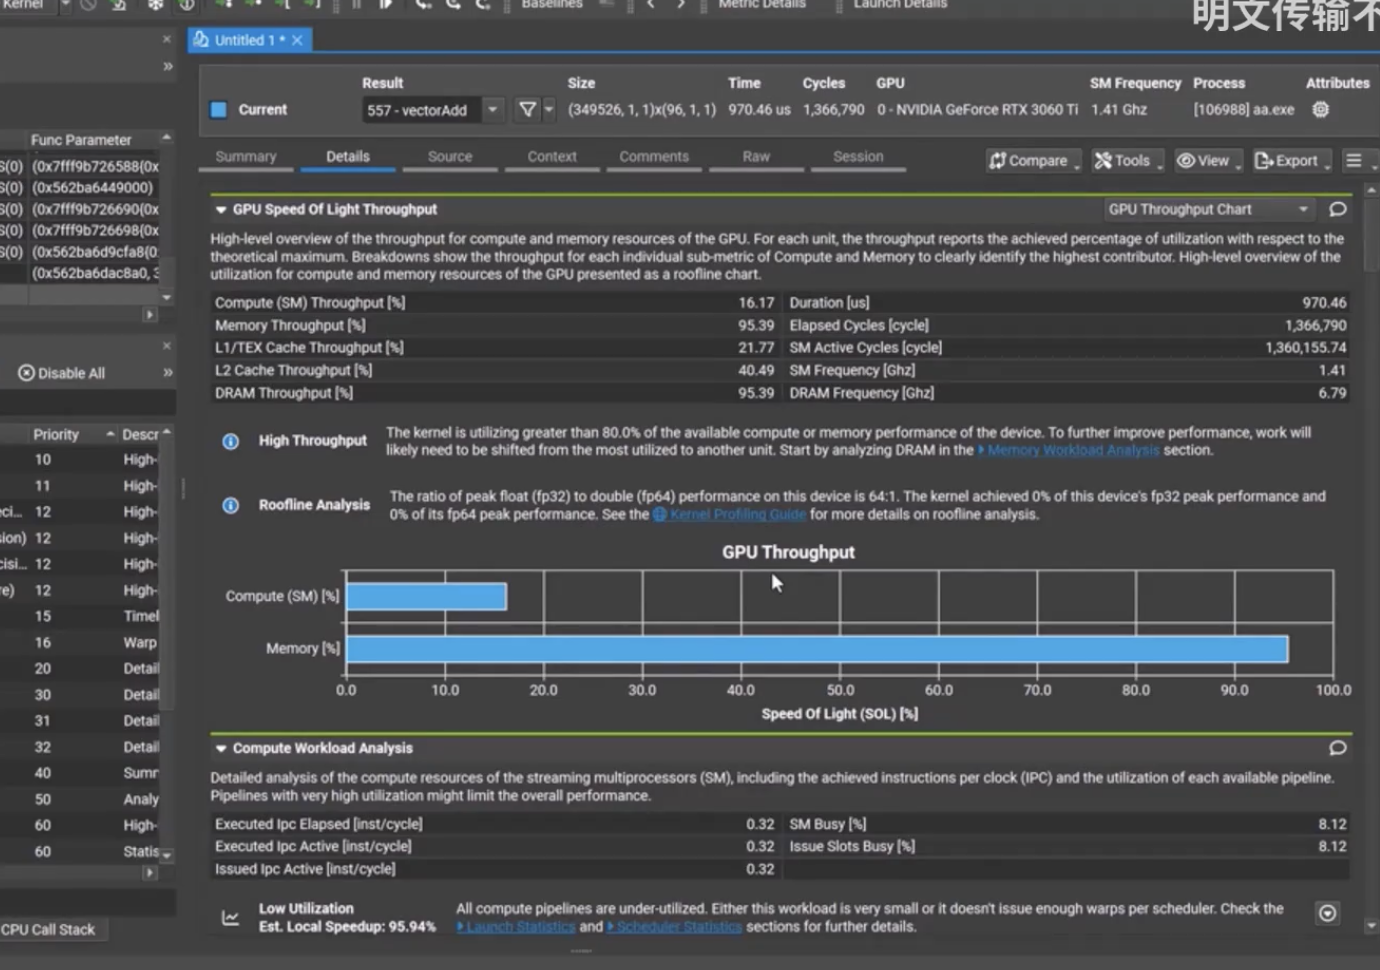
\includegraphics[width=0.75\linewidth]{resources/cuda-109.png}
    \caption{}
    \label{fig:placeholder}
\end{figure}

\subsection{指令依赖与停滞分析}

现在不解释为什么这里两者都有。R4、R3。但想象一下可以把 \texttt{IMAD} 当做 \texttt{ADD} 使用，然后还有 \texttt{ADD}，这是加法过程。读取 B 值并存储在 R3，因为读取 A 值并存储在 R4，然后如所示，在这里将 R4 和 R3 相加，并将值存储在 R9。但不管怎样，现在不想关注这个命令。但能看到这里的感叹号吗？如所示，如果把鼠标移到这里，会看到这个信息。这一行指令要对 84\% 的停滞负责，所有 Sub-warp 停滞的 84\%。

再看一下这一行指令停滞的 99.7\%，这一行指令导致了停滞。可能会问为什么是这一行？这只是加法，为什么加法过程会导致大量停滞？

如所示，有一个依赖，如果不从内存读取两个值，就无法对它们进行加法。这个加法将等待直到从内存获取 R4 和 R3。这就是为什么这里有依赖，这个依赖可以在这里显示出来。确认一下，有这个信息。

是的，如果引用这个指令，这些就是对依赖的解释。这个依赖于这个和这个。每当在这里看到这个，这意味着这个依赖于前面的那个。看看这个指令依赖什么。如果到这里看看这个三角形符号，从汇编代码看，它应该依赖于 R3 和 R4。这是三角形符号。它具体在哪里？是的，这里有一个依赖。

看看这个，看到 R4 了吗？如所示，依赖于 R4。但也应该看到，这里有什么依赖于 R3。

集中在这里，R4 在这里和这里都存在，这个指令需要等待来自这里的 R4，然后这个指令需要等待来自这里的 R4，情况就是这样。还有看看这个，每当看到右侧的这个部分，就会看到依赖关系。例如再次集中注意力，这里有一个向右的箭头，如果向上看会发现它依赖于 R4。这里同样这个指令有另一个向右的三角形。R3 也有一个向右的三角形，它依赖于这里的这个指令。如果点击这里，会发现它也依赖于 R3。如所示 R3，这就是这里展示的依赖关系。

回到这里查看已执行的指令，这是每条指令执行时间的百分比。但可以看看这里的 Warp 停滞采样，可以看到这个指令导致了大约 93\% 的 Sub-warp 停滞。因为它等待前面所有指令的结果，而前面所有指令又依赖于更前面的指令，这是最后一条指令，它依赖于前面的所有指令。

同样对于存储指令，也是因为一旦完成了加法过程或加法操作，需要将值存储到内存中的 C 里。这就是为什么这里有一条存储指令，\texttt{STG} 存储到全局内存。需要从加法过程或加法操作中取出 R9，并将其存储在 C 值中。如所示，同样这条指令导致了 93\% 的停滞。这解释了这里的一切。在 Sub-warp 统计中，看看有什么。

是的，从这些选项中可以确定其他一些选项。例如有地址空间，可以从这里开始查看已执行的指令，但可以专注于地址空间。地址空间意思是在这里访问的是全局内存，但可以左右移动这个来查看所有内容，这也适用于全局内存。如果看这条指令，正在从全局内存加载，这些信息非常重要。

这是加载不是存储，但这里是存储。而扇区（Sector）是一个扇区，这里的扇区大小是 32 字节。因为如果还记得前文，一个扇区等于 32 字节。很多线程不仅仅是相加两个元素，每个是四字节加四字节，正是相加两个元素。但是是针对不同的线程，所以每个线程将需要四字节，这就是为什么每次指令执行加载 32 字节。

是的，这是寄存器的活跃性。还有其他内容吗？不确定活跃寄存器的含义，但可以稍后讨论。如果有其他核函数，可以从这里选择核函数。这里是 SASS，但没有生成 PTX，所以关注的是 SASS 指令，现在先跳过它。上下文，这是稍后需要讨论的内容。

环境（Environment），在这里可能会看到一些关于操作系统的信息。比如 Windows 11 名称、创建时间，拥有的 CPU 主机架构等。如果想查看这些信息，这只是其中一部分。如果 Nsight Compute 图形界面提供了关于性能分析的注释，这里应该包含一些注释，但不需要看这个。

回到详情，看看是否还有其他需要查看的东西。这里有一些说明，如果增加每个线程的寄存器数量会发生什么？实现了大约超过 40\%，好像是 50\% 左右。在纵轴上有 Sub-warp 占用率。这里这个 48\%，这是因为每个线程使用了 16 个寄存器。但它说如果改变应用程序代码来增加每个线程的寄存器数量，将会降低 Sub-warp 占用率，正如这个图所示。这意味着可以从这个图中了解到，可以将每个线程的寄存器数量从 16 增加到 40，而不会导致 Sub-warp 占用率的下降。

这就是需要从这里学习的。可以将每个线程的寄存器数量从 16 增加到 40，而不会导致任何下降或损害 Sub-warp 占用率，这对性能来说是非常重要的。如果将每个线程的寄存器数量增加到超过 40，那么将会导致性能问题。同样适用于块大小——应用程序性能。它说在这里，在这个点上块大小是每个块 96 个线程，使用每个块 96 个线程，可以从这里的启动统计中看到这一点。它说，如果将这个数字从 96 增加到 128，Sub-warp 占用率将不会有任何影响。

这里只讨论 Sub-warp 占用率，但如果到这里将其增加到例如 800，将大大降低占用率，从 48\% 降到大约 24\%，相当于占用率下降了 50\% 左右。但如果例如将其增加到 224，将稍微降低占用率。如果降低了占用率，将会影响应用程序的整体性能。如果增加了使用的共享内存，将会导致占用率的下降。同样适用于每个块的共享内存，但这里是因为在这个应用程序中没有使用共享内存。

不打算再次解释所有这些，但需要看看这部分。这是总数，不是每个 SM。在解释 Warp 停滞采样，并说有 47000 次停滞。它说可以点击这里来了解是哪条指令导致了所有这些停滞。如果还记得从源代码标签页，知道这条指令导致了大部分的停滞。但可以点击这里，它会带我们到同一条指令。

可以从这里的百分比值看到停滞的第二大原因。不知道是否有更多，但可以来到这里点击导致停滞的第二条指令，它会带我们到那个分支。再次点击这里，它选择了这里的这个，因为这个导致了 2\% 的停滞。无论如何，这是针对执行最多的指令。如果点击这里，它会带你去那条执行了一百多万次的指令。点击这里，这条执行了一百多万次，可以对其他的做同样操作，但不全部演示。

\subsection{占用率计算器与优化}

\begin{figure}
    \centering
    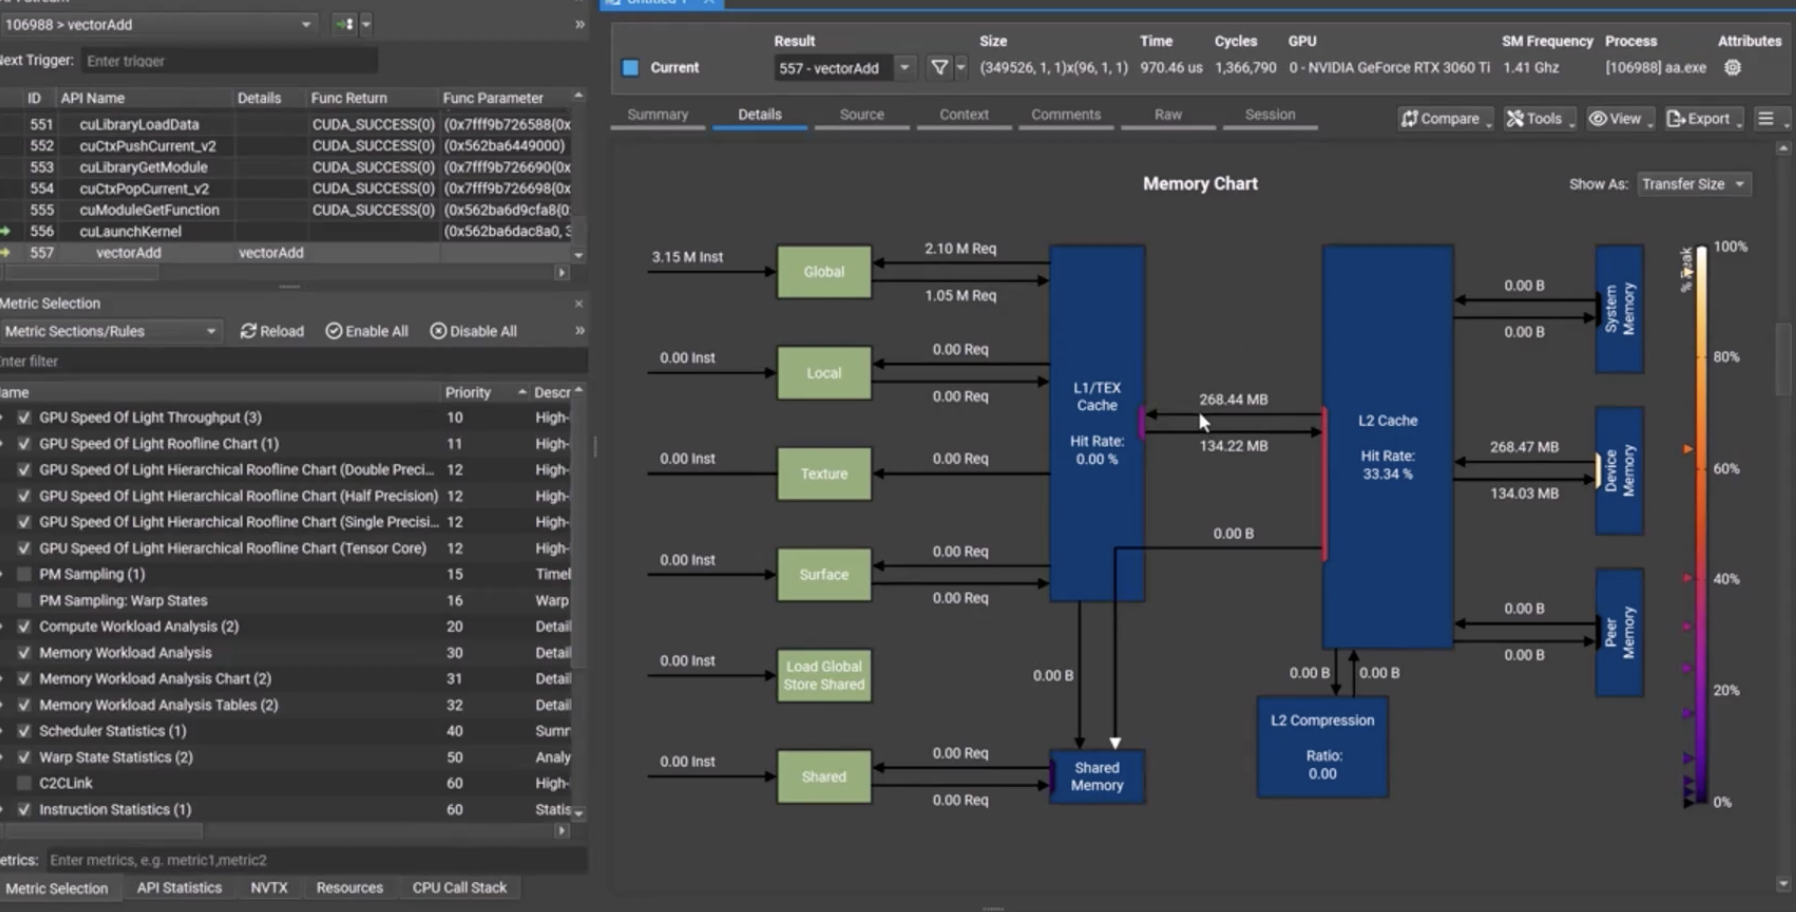
\includegraphics[width=0.75\linewidth]{resources/cuda-110.png}
    \caption{}
    \label{fig:placeholder}
\end{figure}

\begin{figure}
    \centering
    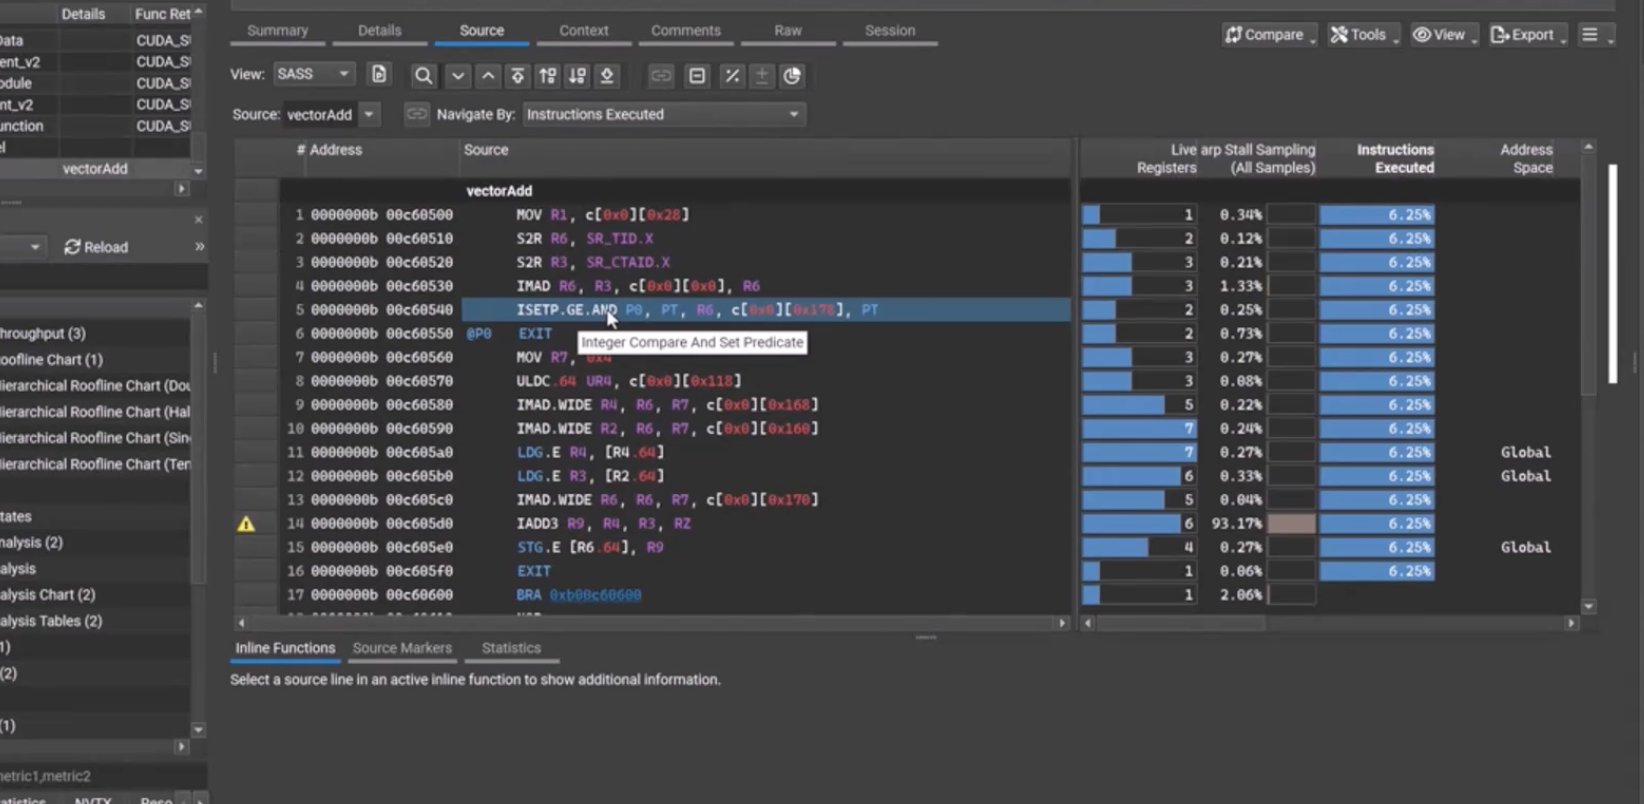
\includegraphics[width=0.75\linewidth]{resources/cuda-111.png}
    \caption{}
    \label{fig:placeholder}
\end{figure}


\begin{figure}
    \centering
    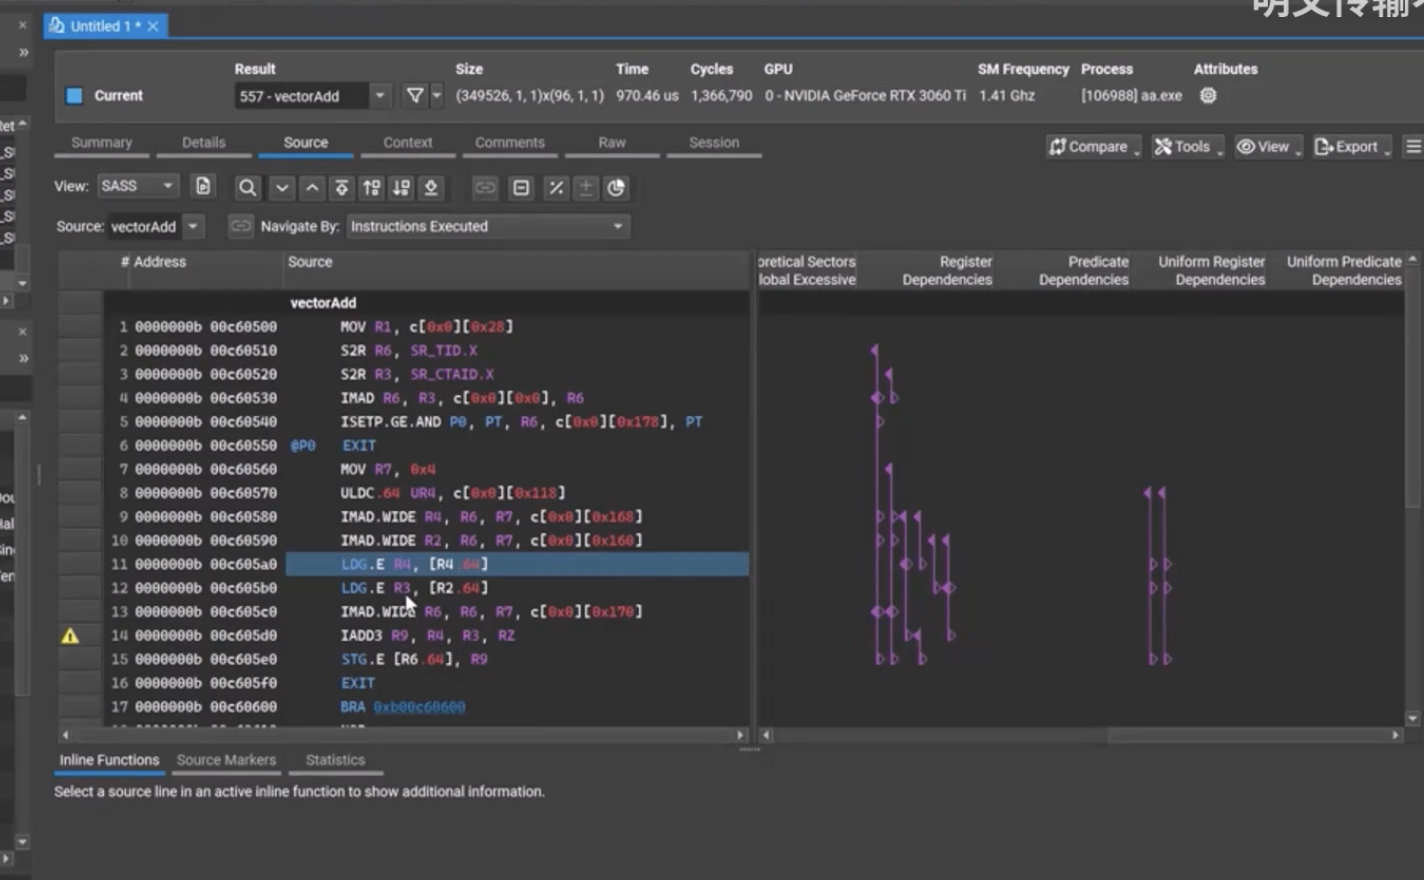
\includegraphics[width=0.75\linewidth]{resources/cuda-112.png}
    \caption{}
    \label{fig:placeholder}
\end{figure}


\begin{figure}
    \centering
    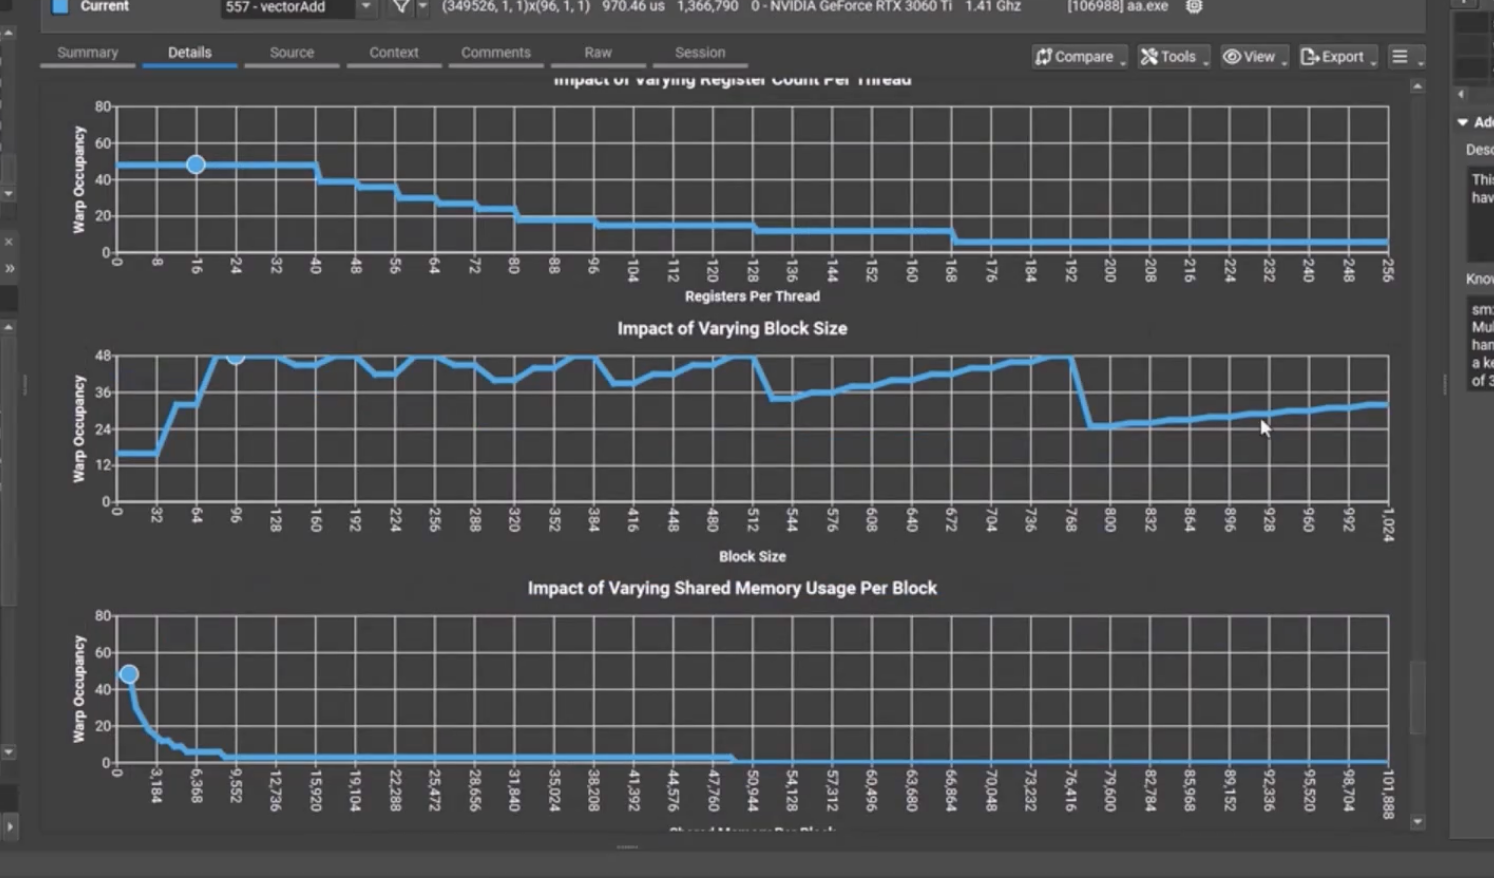
\includegraphics[width=0.75\linewidth]{resources/cuda-113.png}
    \caption{}
    \label{fig:placeholder}
\end{figure}


这就是 Nsight Compute 用户界面的工作方式。关于它就是这样了，只是确认没有其他内容了。是的，这里指标详情这个标签页，当点击这里并点击这里，这会显示任何所选项目的详情。当选择某个项目时，它会把详情显示在这里，然后也可以显示占用率计算器（Occupancy Calculator）。前文讨论过这个计算器以及如何计算占用率。可以在这里修改这些数字，看看它们对占用率的影响。

同样前文在另一个标签页看到的这些图表在这里也有解释，但在这里可以操作它们。可以在这里修改并观察对数值的影响。不确定现在是否有效。是的，它起作用了。比如说 1024，比如说如果点击这里的 256，看到了吗？看到变化了吗？

这也是一个很好的功能，可以看到这些配置对性能的影响。可以折叠各个部分以隐藏图表，只看数字。还有什么功能？然后可以把性能输出在这里，导出或保存为 PDF、图像或其他格式。

可以设定一个基线（Baseline）。如果有一个核函数并想将其与其他核函数进行比较，可以在这里进行比较。可以将一个核函数设定为基线。还能在这里查看什么？从这里开始有一个叫做 API 统计的功能，可以查看或者说隐藏这里的任何部分。从这里这将展示 CUDA 的运行时 API。还记得吗？前文有关于运行时 API 的章节，所以需要看那个章节来理解这里讨论的内容。

\texttt{cudaMemcpy} 操作，这被称为 CUDA 运行时 API。\texttt{cudaMalloc} 在 GPU 的全局内存中分配空间，这也被称为 CUDA 运行时 API。同样适用于在应用程序中使用的所有其他函数，但这非常重要，因为它解释了这些 API 在这个应用程序中各消耗了多少时间。例如仅仅将数据从 CPU 复制到 GPU 或反之，这就消耗了大约 40 毫秒。在 GPU 中分配空间，这大约需要 7 毫秒。同样这与核函数执行无关。这里只是将数据从 CPU 复制到 GPU，而这里再进行分配。还记得这里的指针吗？这显示了曾经执行需要的时间。大约是 7 毫秒，这些 API 需要多少时间？可以看看这些 API 各需要多少时间来执行。

不需要看所有这些东西，只需要关注指标选择和 API 统计。据所知，还可以从这里选择许多其他选项，例如这个显示或隐藏这里的内容。可能需要做的事情之一是，例如添加另一个选择项。这个分析如果想要分析核函数，比如说修改了核函数中的任何内容并想再次分析它，只需点击这里或这里。如果添加了另一个选择项，需要从这里再次分析核函数。

然后从工具菜单有项目资源管理器、输出消息。看看输出消息，没有任何输出消息，也可以看看这里的选项，可以查看诸如字体等选项，这是针对用户界面本身的，可以选择一些配置，轻松地操作这些设置。然后从窗口菜单，可以显示或隐藏这里的一些窗口。

这就是关于 Nsight Compute 工具的图形用户界面的全部内容。但这并不是使用 Nsight Compute 工具的结束。因为当开始讲解性能章节和优化时，将基于从 Nsight Compute 获得的结果进行优化。
